\documentclass{qualitätssicherungsheft}
% glossary
\makeglossaries

\begin{document}
\newglossaryentry{label}{
    name=Label,
    plural=Labels,
    description={Rezepte können mit bezeichnenden Stichwörtern, sogenannten Labels, versehen werden. Dies ermöglicht das Filtern von Rezepten nach bestimmten Eigenschaften (z.B. vegetarisch, glutenfrei, halal)}
}
\maketitle
\tableofcontents
\newpage

\section*{Gender-Hinweis}
Zur besseren Lesbarkeit wird in diesem Entwurfsheft das generische Maskulinum verwendet.
Die in diesem Heft verwendeten Personenbezeichnungen beziehen sich - sofern nicht anders kenntlich gemacht - auf alle Geschlechter.
\newpage

\section{Gefundene Fehler}
In diesem Abschnitt werden während der Qualitätssicherungsphase gefundene Fehler dokumentiert.

\subsection{Fehler 1}
Beschreibung: Server gibt bei Fehler immer 500 zurück. \newline
Entdeckt durch: Integrationstests \newline
Fix: Fehler in Errorhandler behoben.

\subsection{Fehler 2}
Beschreibung: Server gibt bei Erstellen von Gruppe und anschließendem Löschen anschließend an jedem Endpunkt Fehler 502 aus \newline
Entdeckt durch: Tester Henri Becker \newline
Fix: 

\section{Tests im Backend}
Das Backend wurde mit Integrationstests getestet. Die Tests wurden mit dem Framework Mocha geschrieben. 
Die Tests sind in dem Ordner \textit{test} zu finden. Die Tests können mit dem Befehl \textit{npm test} ausgeführt werden.

\section{Nichtfunktionale Anforderungen}
\subsection{Änderbarkeit}
Die Änderbarkeit des Backends wurde durch die Verwendung von TypeScript und der Verwendung von REST-API sichergestellt.
Durch die Verwendung von Controllern mit dehr niedriger Kopplung ist eine Änderung oder Erweiterung der Funktionalität des Backends einfach möglich.

\subsection{Sicherheit}
Die Sicherheit des Backends wurde durch die Verwendung von Firebase sichergestellt. 
Dieses bietet als Google-Service eine sichere Nutzer- und Sessionverwaltung.

\section{Lasttests}
Da unsere Anwendung auf die Verwendung vieler Nutzer ausgelegt ist, haben wir Lastentests durchgeführt.
Diese wurden mit dem Tool Artillery durchgeführt.
Die Testumgebung sah dabei wie folgt aus:
Wir haben unsere Backend auf einem Server mit nahezu identischer Hardware wie der Server, auf dem die Anwendung später laufen soll, deployed.
Der Server besaß 2 vCores und 4 GB RAM.
Der Server der Anwendung besitzt 2 vCores und 2 GB RAM.
(Leider konnten wir im Rahmen des PSE keine bessere Testumgebung bereitstellen ohne auf monetär Mittel zurückzugreifen.)

Der Test bestand aus drei aufeinanderfolgenden Phasen.
In jeder Phase wurde die Anzahl der virtuellen Nutzer dabei Stufenweise im 10 Sekunden Intervall im Testzeitraum erhöht.
\begin{itemize}
    \item In der ersten Phase wurden für 60 Sekunden jede Sekunde 1 bis abschließend 5 virtuelle Nutzer erstellt.
    \item In der zweiten Phase wurden für 60 Sekunden jede Sekunde 5 bis abschließend 15 virtuelle Nutzer erstellt.
    \item In der letzten Phase wurden für 20 Sekunden jede Sekunde 15 bis abschließend 25 virtuelle Nutzer erstellt.
\end{itemize}

Die drei Phasen sollen dabei einmal ein leichtes bis normales, ein normales bis hohes und ein spitzen aufkommen von Anfragen simulieren.

Jeder Nutzer hatte im Test die selbe Aufgabe.
Er Nutzer sollte sich
\begin{itemize}
    \item einloggen
    \item alle Rezepte aufrufen
    \item einer Gruppe beitreten
    \item Namen von Zutaten aufrufen
    \item ein Rezept erstellen
    \item die Rezepte nach betrete der Gruppe erneut aufrufen
    \item und anschließend  und ein Bild aufrufen.
\end{itemize}
Mit diesem Ablauf haben wir versucht, die Anwendung mit einer realistischen Nutzung zu testen, die aus den Kernfunktionen der Anwendung besteht.
Dadurch, dass die Nutzer alle der gleichen Gruppe beitraten und ein Rezepte erstellten wurde das aufkommen der Anfragen über den Verlauf des Tests hinweg immer größer.
Damit konnten wir sicherstellen, dass die Anwendung auch bei großen Anfragen stabil bleibt.

\subsection{Bemerkung zur Aussagekraft der Ergebnisse}
Leider konnten wir unseren Test nur in einem limitierten Umfang durchführen.
Grund dafür war, dass unser Server leider zu wenig Rechenleistung besaß, um die Anfragen von vielen Nutzern zu verarbeiten.
Wir kamen so schon bei denn doch noch vergleichsweise geringen Nutzern in unserem Test an die komplette Auslastung des Servers und konnten so nicht exakt analysieren, wie unsere Anwendung sich bei einem hohen aufkommen von Anfragen verhält.
Deshalb sind die Ergebnisse des Tests nur bedingt aussagekräftig.

\subsection{Metriken}
Für die Auswertung des Tests haben wir uns auf zwei Metriken konzentriert.
Einmal die Median Antwortzeit und einmal den Apdex-Wert.
Die Median Antwortzeit gibt an, wie lange eine Anfrage im Median benötigt hat, um beantwortet zu werden.
Apdex (Application Performance Index) ist ein standardisiertes Maß zur Bewertung und Berichterstattung über die Zufriedenheit der Benutzer mit der Leistung von Anwendungen und Diensten. Es bietet einen einfachen, verständlichen Überblick über die Nutzerzufriedenheit und ist besonders nützlich für solche, die eine schnelle Einschätzung der Anwendungsperformance benötigen, ohne sich mit detaillierten Metriken auseinandersetzen zu müssen.

Der Apdex-Wert wird als Zahl zwischen 0 und 1 ausgedrückt, wobei:
\begin{itemize}
    \item 1 eine vollständige Zufriedenheit der Benutzer darstellt.
    \item 0 vollständige Unzufriedenheit der Benutzer bedeutet.
\end{itemize}

Dabei wird die Zeit in drei Bereiche eingeteilt.
Anfragen, die innerhalb einer bestimmten Zeit beantwortet wurden, werden als zufriedenstellend gewertet.
Anfragen, die länger als die bestimmte Zeit benötigen, werden als nicht zufriedenstellend gewertet.
Anfragen, die innerhalb der bestimmten Zeit beantwortet wurden, werden als tolerierbar gewertet.
Der Apdex-Wert ist dann der Anteil der zufriedenstellenden und tolerierbaren Anfragen an allen Anfragen.

Bei unserem Test haben wir uns für einen Schwellwert von 1.9 Sekunden entschieden. Wir haben uns für diesen Wert entschieden, da wir der Meinung sind, dass eine Anfrage, die länger als 1.9 Sekunden benötigt, nicht mehr zufriedenstellend ist. Hinsichtlich dem aufkommen von Daten, die wir bei Anfragen erwarten, ist dies in unseren Augen ein realistischer Wert.

\subsection{Ergebnisse}
In unserem Test erziehlten wir bei einem Apdex-Wert von 1.9s und einer Median Antwortzeit von 0.4879 Sekunden einen Score von 0.84. Damit wird die Anwendung als zufriedenstellend bewertet.

\begin{figure}[!htp]
    \centering
        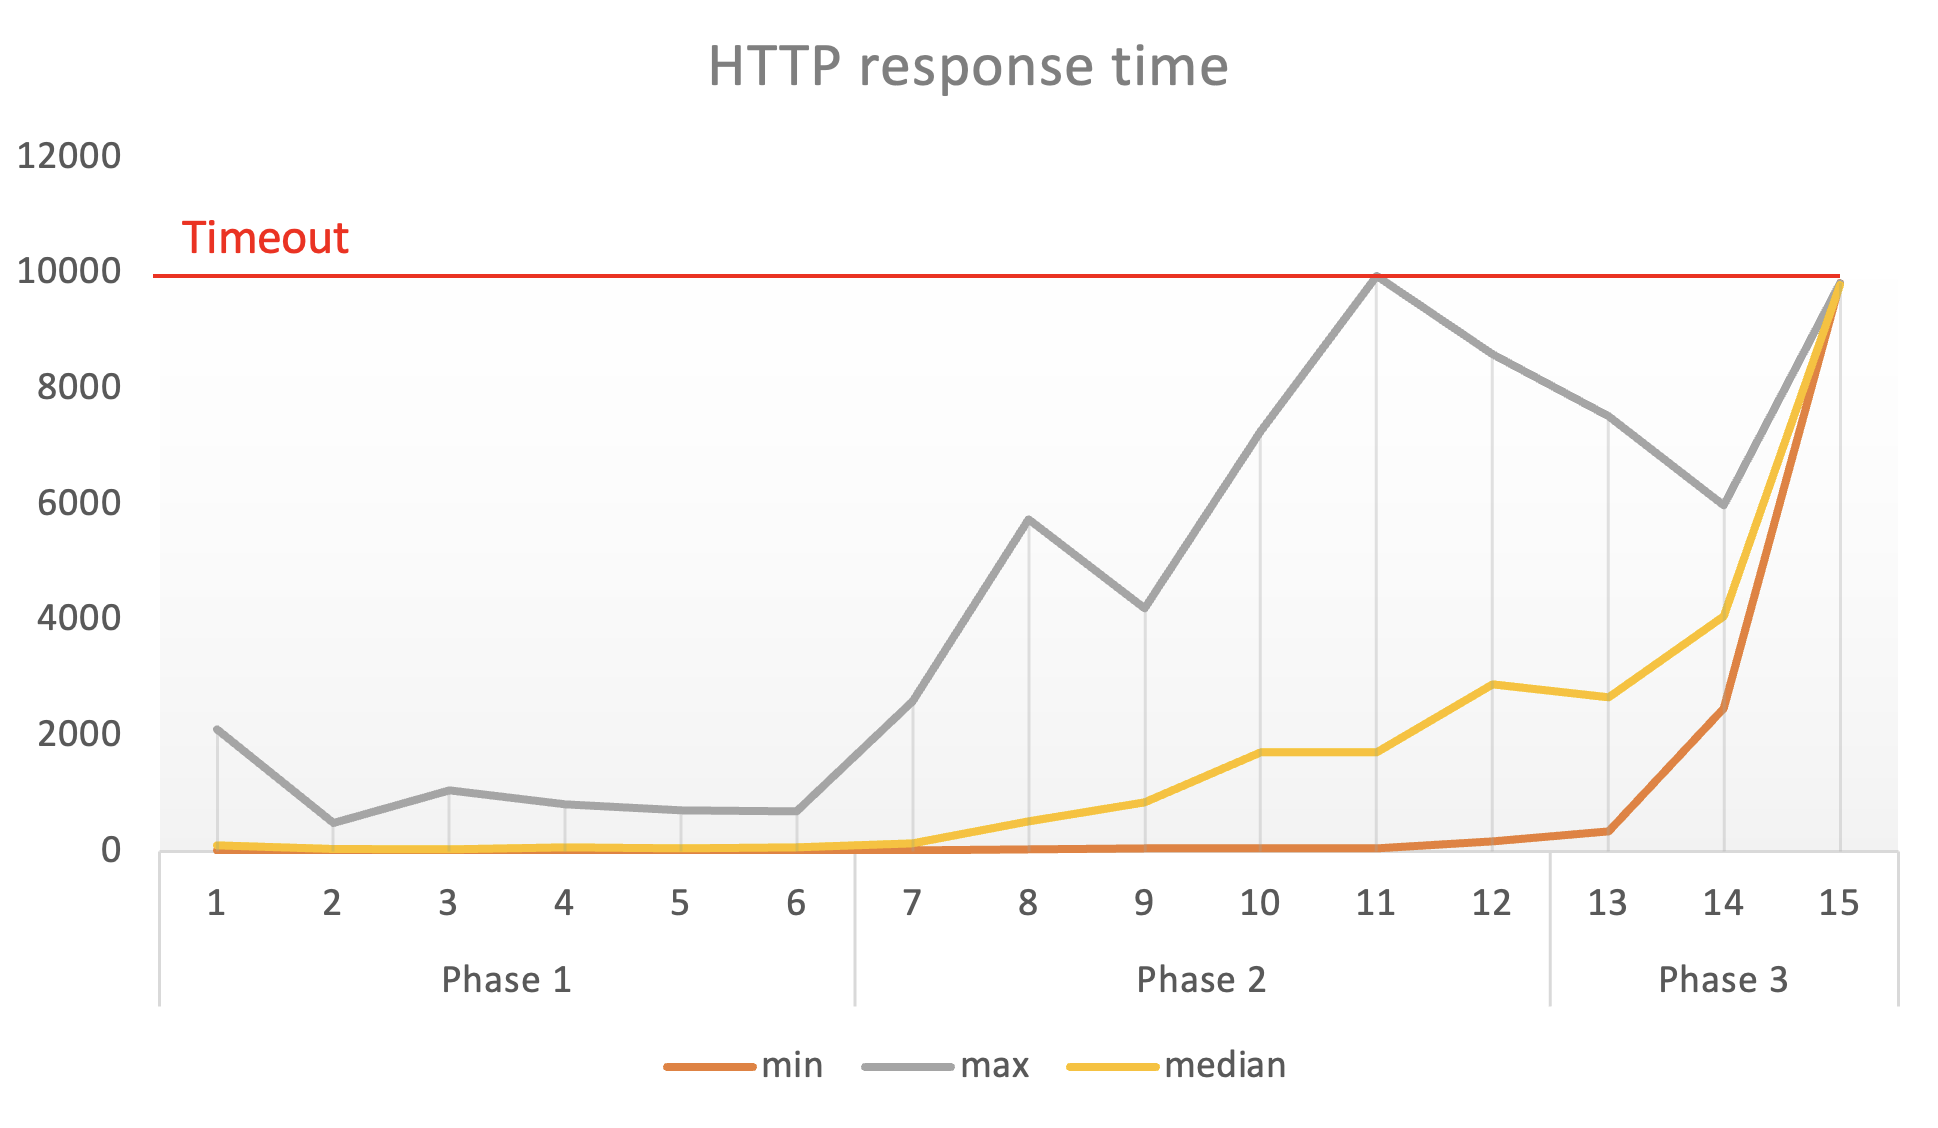
\includegraphics[height=80mm]{images/lasttest/response_time.png}
        \caption[center]{HTTP Response Time}
        \label{fig:http_response_time}
\end{figure}

Wie man in der Abbildung \ref{fig:http_response_time} sehen kann, steigt die Antwortzeit mit der Anzahl der Nutzer an. Was zu erwarten war. Was jedoch auch auffällt, dass ab der dritten Phase die Antwortzeit über unsern Schwellwert von 1.9 Sekunden steigt. Dies ist darauf zurückzuführen, dass der Server nicht mehr in der Lage war, die Anfragen zu verarbeiten. Dies ist auch in der Abbildung \ref{fig:cpu_usage} zu sehen. Die CPU-Auslastung steigt mit der Anzahl der Nutzer an und erreicht schon am Ende der zweiten Phase 100\%. Dies ist auch der Grund, warum wir den Test nicht mit mehr Nutzern durchführen konnten und somit der Test, vor allem zum Ende hin, nur bedingt aussagekräftig wird.

In der letzten Phase ist zu sehen, dass die Antwortzeit weiter bis an die 10 Sekunden steigt. An diesem Zeitpunkt wird eine Anfrage als Timeout eingestuft. Der Test wies dabei 851 Timeouts auf. Das ist leider ein sehr hoher Wert. Dies ist jedoch aus unserer Sicht vor allem auf die geringe Rechenleistung des Servers zurückzuführen. 

Es kam beim gesammten Test nicht zum Absturz der Anwendung.
Jedoch war bei einem versuch mit höheren virtuellen Nutzerzahlen der Server nicht mehr in der Lage, die Anfragen zu verarbeiten und wurde vom Serverbetreiber aufgrund von Überlast neugestartet.

\begin{figure}
    \centering
        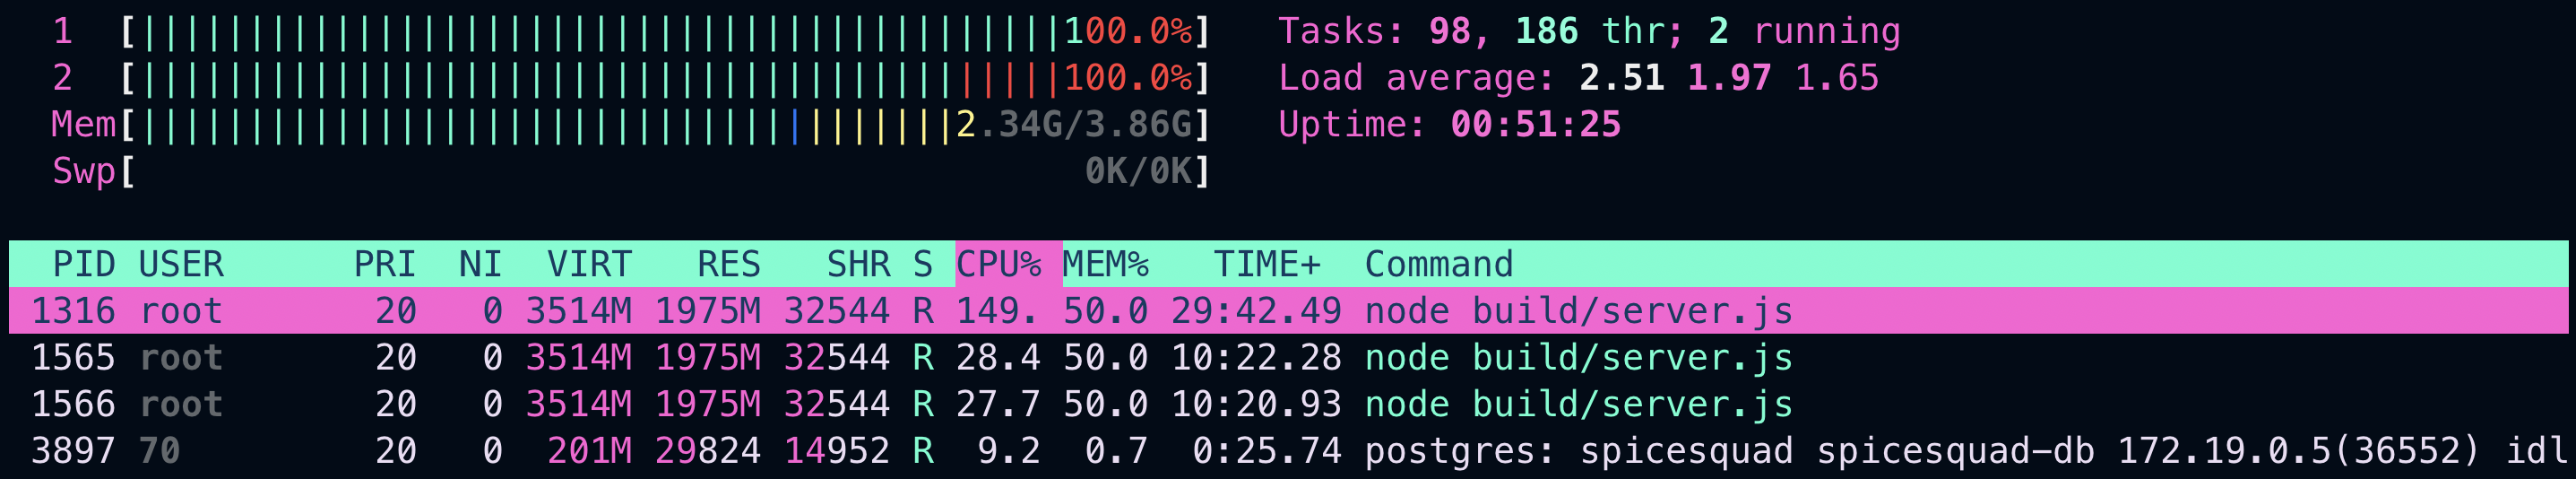
\includegraphics[height=30mm]{images/lasttest/cpu_usage.png}
        \caption[center]{CPU Usage}
        \label{fig:cpu_usage}
\end{figure}

\subsection{Fazit}
Der Test hat gezeigt, dass die Anwendung bei einer geringen Anzahl von Nutzern gut funktioniert. Jedoch wäre die Anwendung nach dem obigen Testergebnis nicht für eine große Anzahl von Nutzern ausgelegt. Dies ist aus unserer Sicht vor allem auf die geringe Rechenleistung des Servers zurückzuführen. Wir sind der Meinung, dass die Anwendung bei einer höheren Rechenleistung des Servers auch bei einer höheren Anzahl von Nutzern gut funktionieren würde.

Um diese Aussage zu bestätigen, müsste jedoch ein weiterer Test mit einer höheren Rechenleistung des Servers durchgeführt werden, was uns leider im Rahmen des PSE nicht möglich war.

\end{document}